\chapter{Implementation of High-fidelity Prototype} \label{chap:impl}
In the previous chapter, we concluded that maps and colors are promising visualizations, and we expressed our interest in further investigating directional indicators. In this chapter, we describe the application we created for the Microsoft HoloLens to test our visualizations in real life. In the next chapter, we will use this application to evaluate our visualizations through on-site user tests.



We developed our application in Unity, which is Microsoft's recommended engine for creating HoloLens applications. Coding was done in C\# using Visual Studio. The project included the \textit{MixedRealityToolkit} \cite{Microsof99:online}, a collection of commonly used scripts and components for creating mixed reality applications, provided by Microsoft themselves. Using this package, setting up a HoloLens project is fairly straightforward, and functionality like gesture control and spatial mapping is quick to implement. We also included Vuforia, a popular AR framework, for its ability to recognize markers in the real world and anchor virtual objects to them.

For the actual user tests, we created a rough virtual copy of our work environment, as shown in Figure \ref{fig:model}. This copy included our office, the neighboring room (which is also the classroom from our online survey) and the hallway connecting the two. We modelled only the relevant components, being the walls, the light switches and the lights themselves. This way, we could highlight these components at will through the augmented view of the HoloLens. The entire environment was anchored to a Vuforia marker, an image taped to the wall in our office. By looking at the image, the HoloLens could determine its location and place the virtual environment precisely on top of the real one. Calibration had to be done only once, at startup, after which tracking worked well enough to let us walk around freely throughout the rooms for extended periods of time.

\begin{figure}
    \centering
    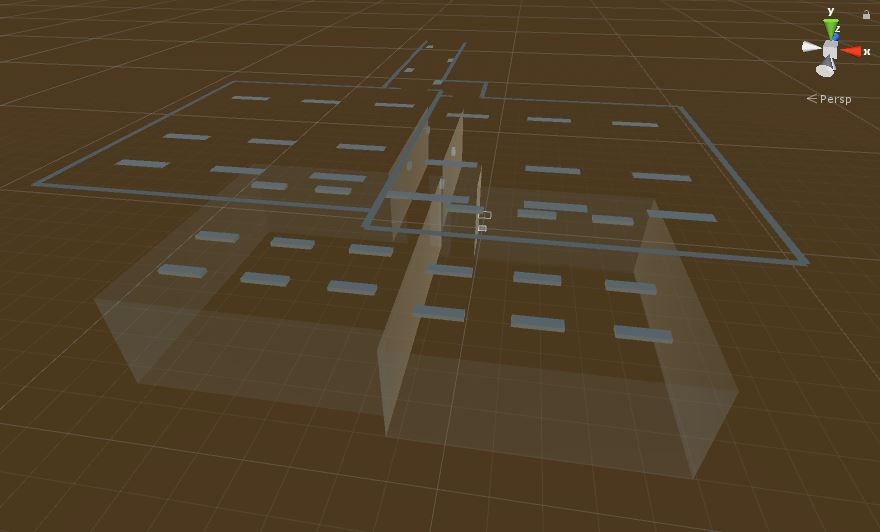
\includegraphics[width=0.8\linewidth]{resources/implementation/model.jpg}
    \caption{View of the scene in the Unity editor.}
    \label{fig:model}
\end{figure}

The two rooms both contain three circuits, each having one switch and three lights. The switches are arranged in a row next to the door, in an unintuitive order, as mentioned in Chapter \ref{chap:explor}. The hallway contains only a single circuit, consisting of two switches that both control the same four lights. The walls and lights have an outline of themselves hovering above the environment. A second Unity camera is anchored to the location of the user and looks straight down on this outline, rotating and shifting with the user, creating a minimap view that we can display in the bottom right of the user's vision. The color of the virtual components and their outlines in the minimap can be controlled separately.

Switches can be selected by gazing at them and then making the tapping gesture or using the HoloLens Bluetooth clicker. A selected switch turns red, as shown in Figure \ref{fig:selection}, and can be deselected by clicking it again. This way, the user can activate visualizations for a specific switch, which will show the lights connected to it. The walls are semi-transparent, allowing users to see the overlay of lights and switches in neighboring rooms, and thus also allowing for visualizations to work across multiple rooms.

\begin{figure}
    \centering
    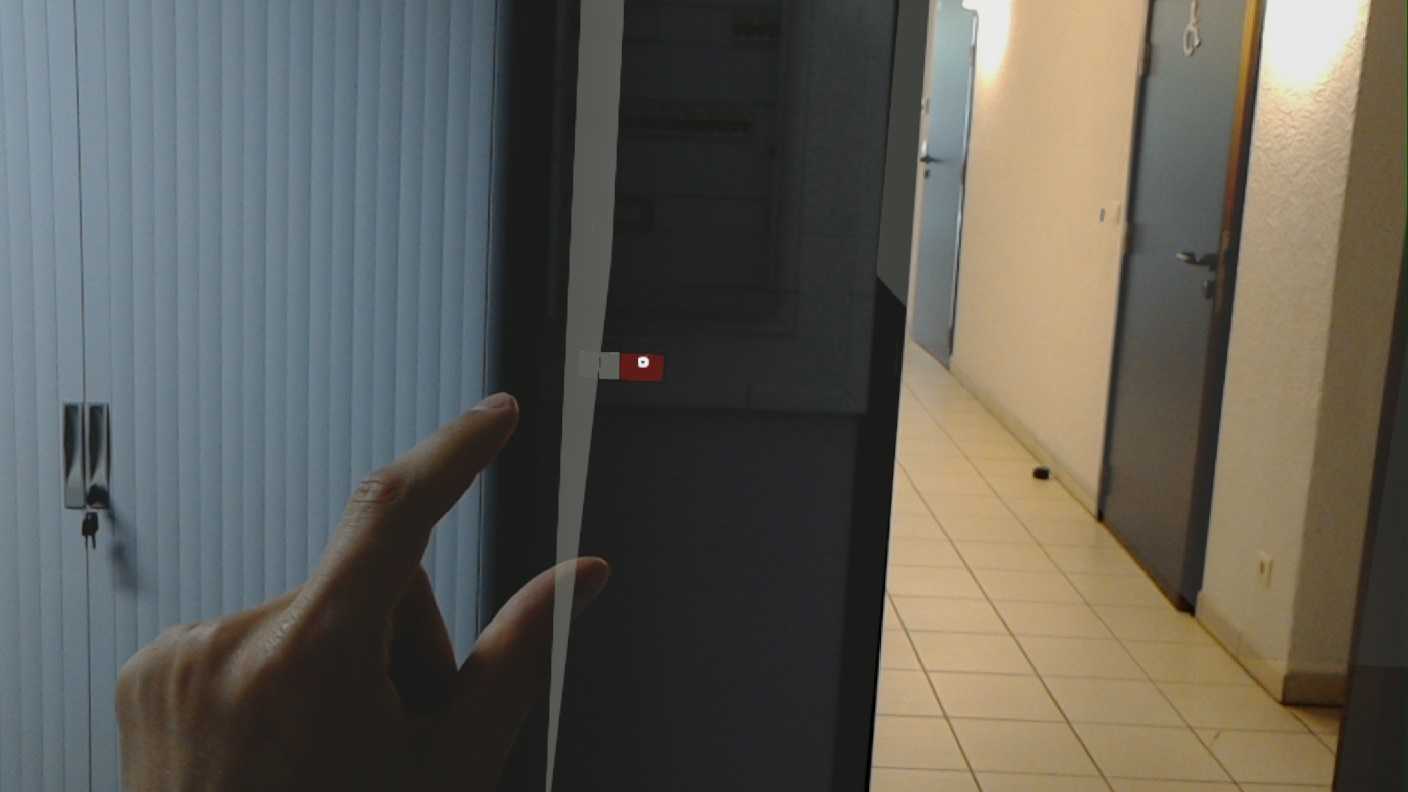
\includegraphics[width=1.0\linewidth]{resources/implementation/selection.jpg}
    \caption{The user selects a switch. The thin white plane is the overlay of a wall further ahead.}
    \label{fig:selection}
\end{figure}

The first visualization that we implement is called the \textbf{world highlights}, because it highlights components in the user's environment. When the user selects a switch, the overlay of the connected lights turn red, as shown in Figure \ref{fig:world_highlights_vis}. The user has no indication of how many connected lights there are and receives no hints as to where they are located; they have to look directly at each light to be able to find them all. We intend this visualization to complement others, rather than stand alone.

\begin{figure}
    \centering
    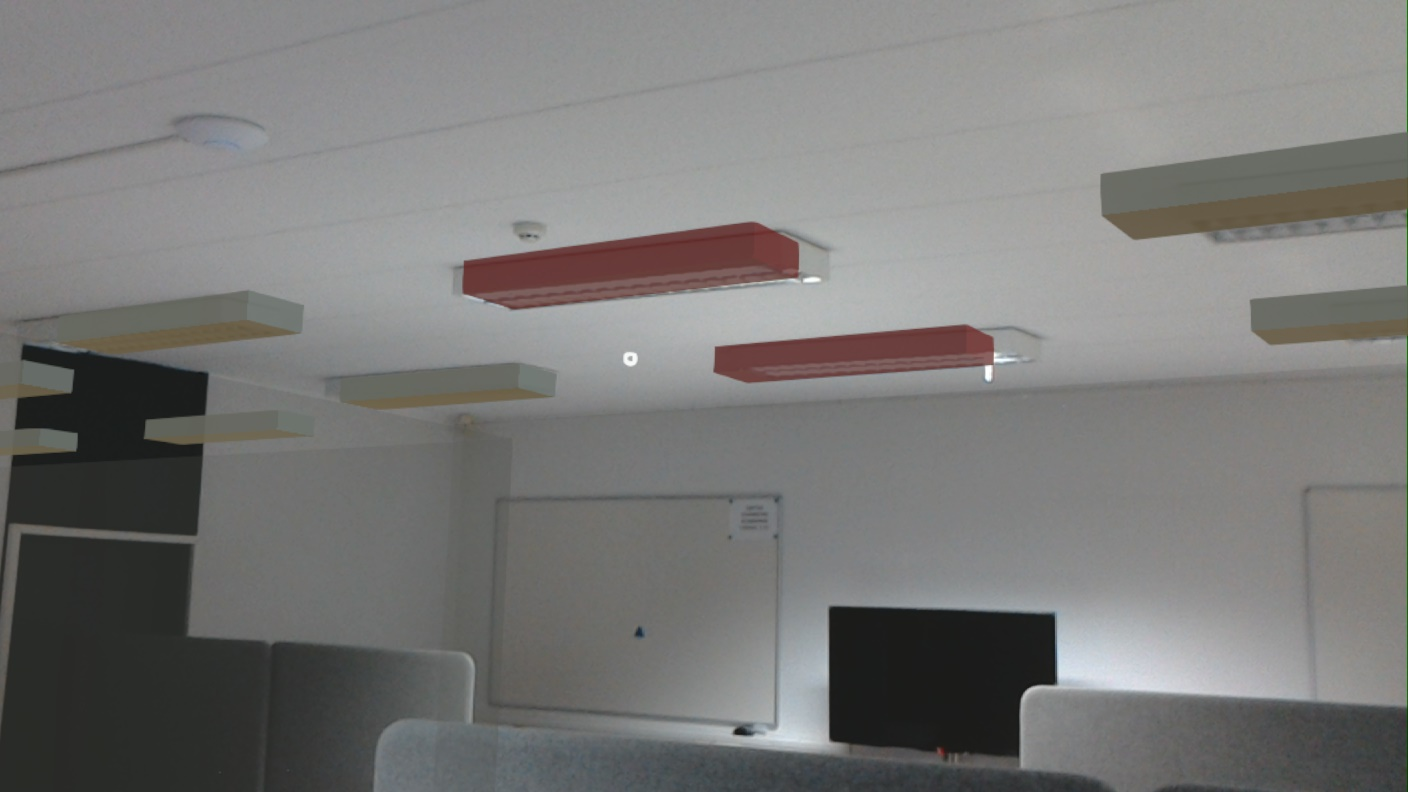
\includegraphics[width=1.0\linewidth]{resources/implementation/world_highlights.jpg}
    \caption{The \textit{world highlights} visualization. On the left, we can see some lights of the neighboring room.}
    \label{fig:world_highlights_vis}
\end{figure}

Our second visualization is the \textbf{minimap highlights}, which highlights the connected lights on a minimap in the bottom right corner of the user's view, rather than directly in the user's environment, and is shown in Figure \ref{fig:minimap_highlights_vis}. The user's location is symbolized by the white diamond in the center. The choice of this visualization is based directly on the popularity of the map visualization in our online survey. The minimap rotates with the user, so that the up side is always the direction where the user is looking at, and it shifts to keep the user centered. The map adds a cognitive step in the light finding process, but it may remove the need for the user to look around once they are familiar with the environment.

\begin{figure}
    \centering
    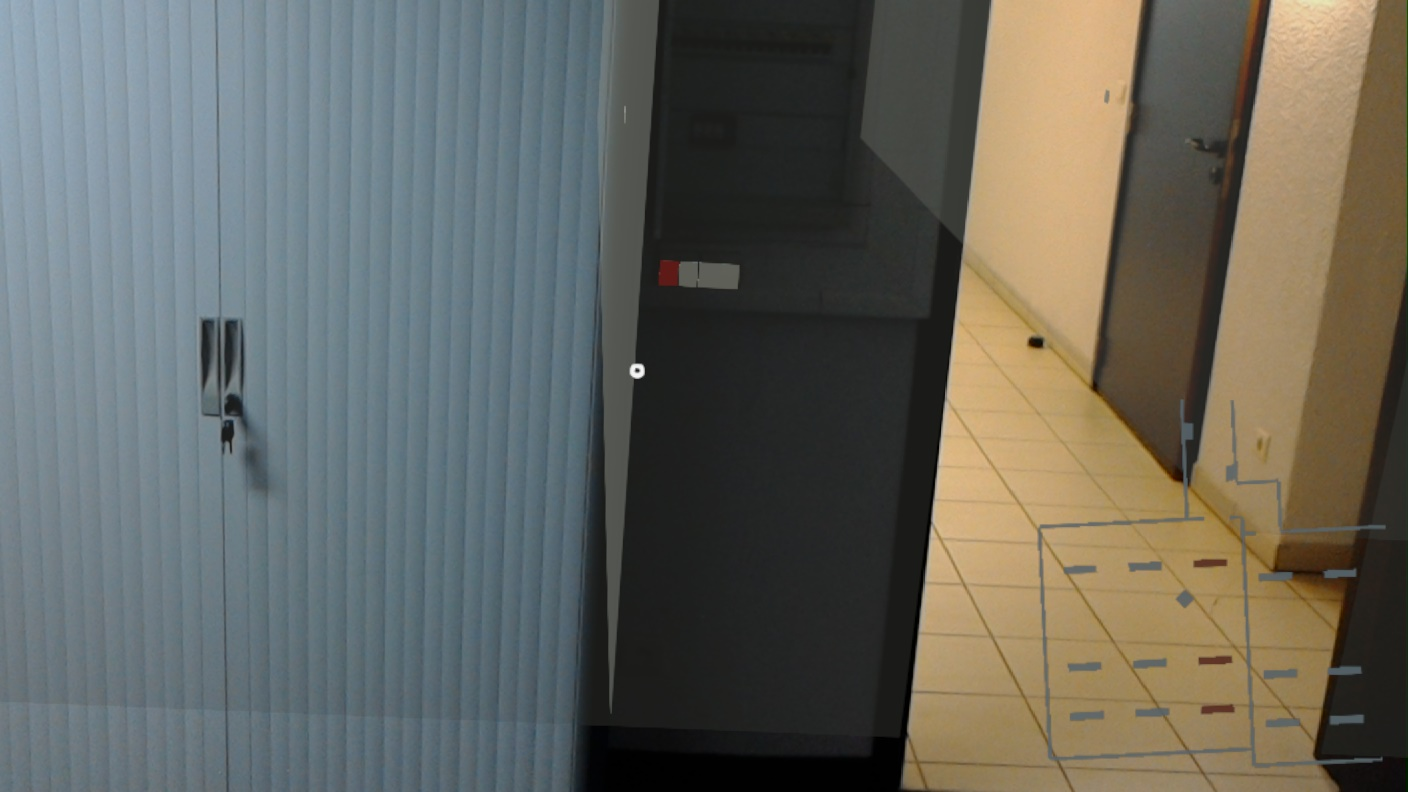
\includegraphics[width=1.0\linewidth]{resources/implementation/minimap_highlights.jpg}
    \caption{The \textit{minimap highlights} visualization. We can quickly tell there are three connected lights, and we could point to them without looking up.}
    \label{fig:minimap_highlights_vis}
\end{figure}

The third and fourth visualization are directional indicators, which we were eager to evaluate in a more high-fidelity setup. First we create the \textbf{arrows} visualization, shown in Figure \ref{fig:arrows_vis}, which creates triangles pointing at each connected light. When the target is outside the field of view, only the base of the triangle is visible in the periphery. The further away the target is, the longer the triangle and so the more parallel the two legs appear. Since all triangles are always visible, the number of connected lights can quickly be counted. The triangles continually adjust while the user looks around, guiding their gaze towards the targets.

\begin{figure}
    \centering
    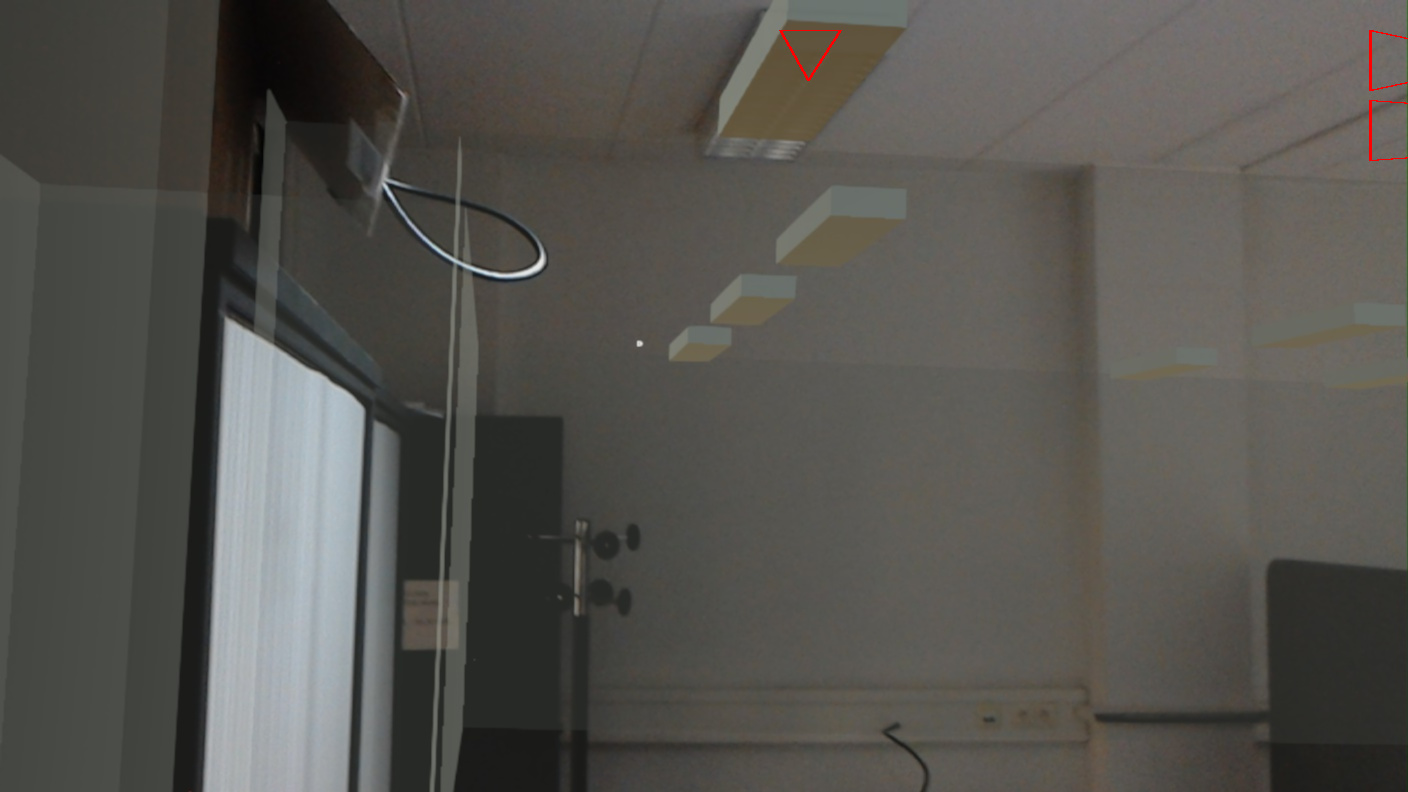
\includegraphics[width=1.0\linewidth]{resources/implementation/arrows.jpg}
    \caption{The \textit{arrows} visualization. We can tell there are two more lights to the right, one close and one further away.}
    \label{fig:arrows_vis}
\end{figure}

The second directional indicator, and the fourth visualization, is the \textbf{halo's}, which we already used in the online survey. They work exactly like the arrows, but use circles rather than triangles, as shown in Figure \ref{fig:halos_vis}. The curve of the lines in the peripheral vision shows us the size of the circles, and thus how far away the targets in their center are.

\begin{figure}
    \centering
    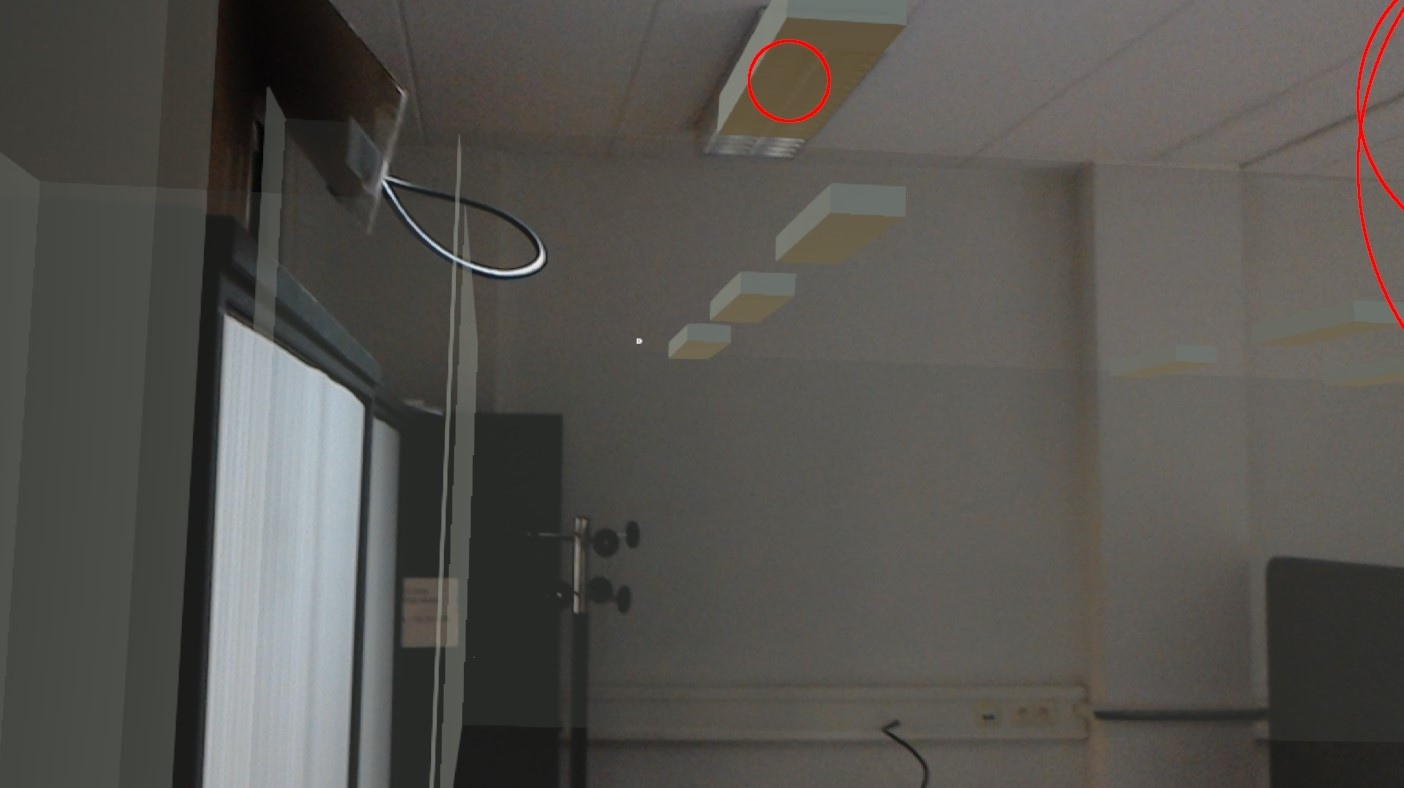
\includegraphics[width=1.0\linewidth]{resources/implementation/halos.jpg}
    \caption{The \textit{halo's} visualization. We can tell there are two more lights to the right, one close and one further away.}
    \label{fig:halos_vis}
\end{figure}

Our fifth and last visualization is the \textbf{colors}, the most promising approach according to our online survey. For this visualization, no switch has to be selected; all circuits are outlined at once, each in their own color, both in the environment and on the minimap, as shown in Figure \ref{fig:colors_vis}.

\begin{figure}
    \centering
    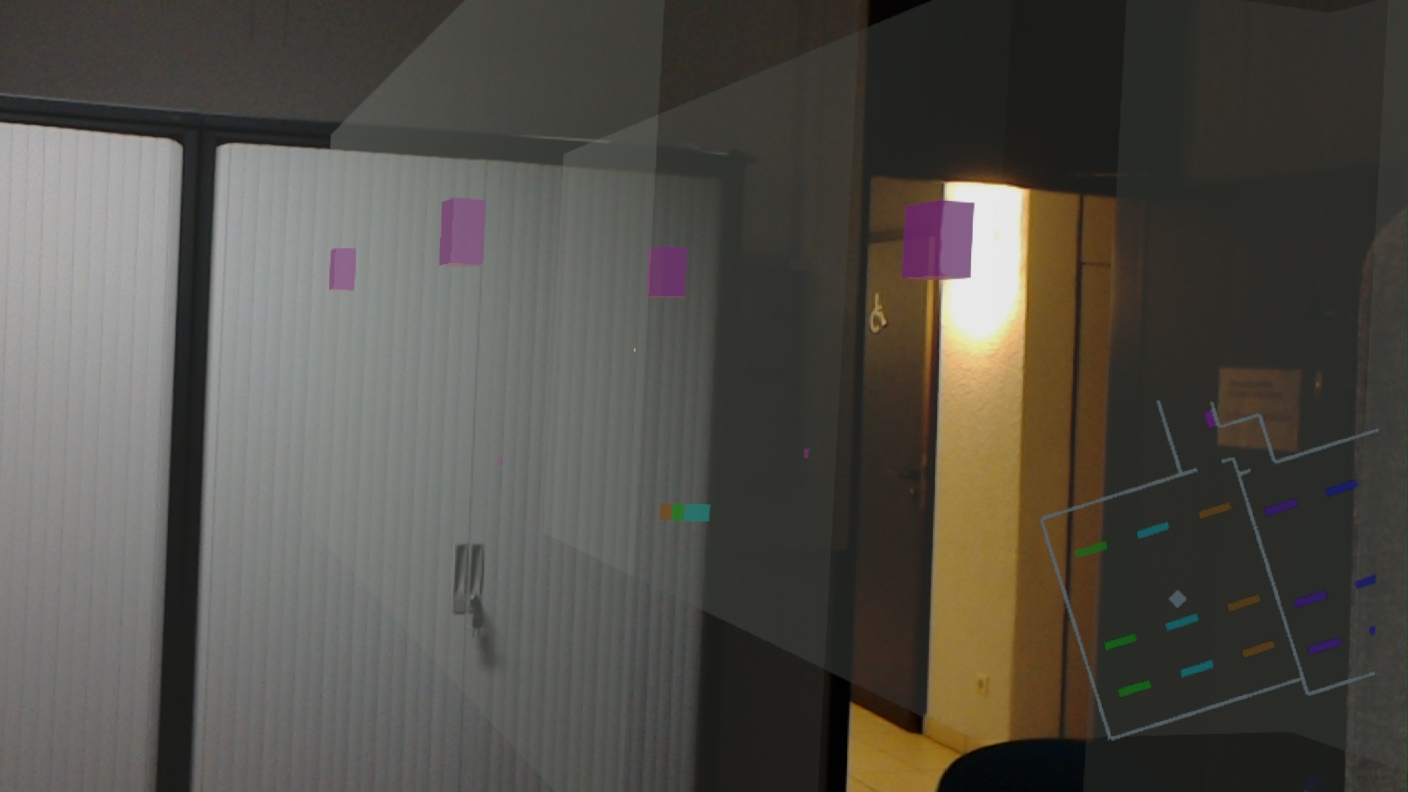
\includegraphics[width=1.0\linewidth]{resources/implementation/colors.jpg}
    \caption{The \textit{colors} visualization. We can find the corresponding lights for multiple switches at once, even in different rooms, by using the minimap or by looking through walls.}
    \label{fig:colors_vis}
\end{figure}

Our application is not limited to using only one visualization at a time; multiple visualizations can be combined to evaluate how they might complement each other. Figure \ref{fig:combo_vis} illustrates this with a combination of the minimap highlights and the arrows. For our user tests, we can remotely control which visualizations are active via the Windows HoloLens application. This application can stream keyboard input from a computer to the HoloLens. Our application listens for these key presses and changes the active visualizations accordingly.

\begin{figure}
    \centering
    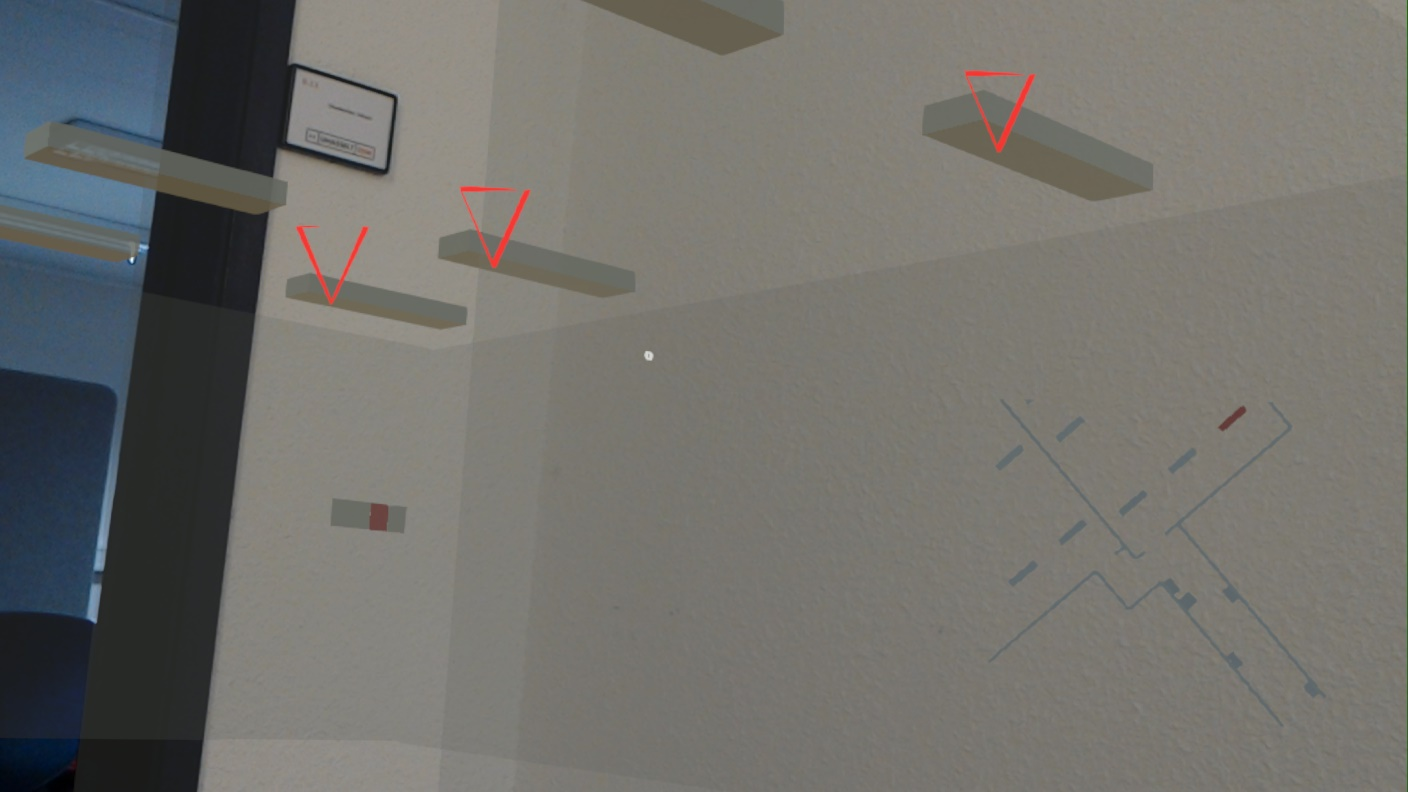
\includegraphics[width=1.0\linewidth]{resources/implementation/combo.jpg}
    \caption{A combination of arrows and minimap highlights. We can see the switches and lights through the wall, and we can compare with the minimap.}
    \label{fig:combo_vis}
\end{figure}
